\documentclass[11pt,a4paper]{article}
\usepackage[margin=1in]{geometry}
\usepackage{amsmath,amssymb}
\usepackage{booktabs}
\usepackage{graphicx}
\graphicspath{{../figures/anchor_29359/}{../figures/comparisons_20260923/}}
\usepackage[hidelinks]{hyperref}

% The document is table-dense, so the default float fractions push a
% full-width figure several pages past the text that discusses it.
\renewcommand{\topfraction}{0.9}
\renewcommand{\bottomfraction}{0.7}
\renewcommand{\textfraction}{0.1}
\renewcommand{\floatpagefraction}{0.7}
\setcounter{topnumber}{3}
\setcounter{totalnumber}{4}

\newcommand{\relltwo}{\ensuremath{\mathrm{relL2}}}

\title{Diagnosing Late-Time Accuracy Limits of Single-Shot Acoustic Neural Operators in Heterogeneous Media}

\author{}
\date{2026-09-23}

\begin{document}
\maketitle

\begin{abstract}
Fast acoustic wavefield prediction requires accuracy in the scattered coda as well as the
first arrival. We study this requirement in a 39.1-million-parameter single-shot neural
operator for heterogeneous two-dimensional media. Our contribution is an auditable diagnostic
protocol combining time- and frequency-resolved error, correction-direction probes, and
controlled intervention tests. On frozen training panels, full-future relative $L^2$ is
$0.0609$, $0.2303$, and $0.3965$ for uniform, layered, and Marmousi media, respectively.
For Marmousi, the final time third contains $64.1\%$ of the mean per-record error share but
only $30.6\%$ of the corresponding signal-energy share. None of its 96 records reaches
$0.1$. A preregistered 18,700-step intervention increases late-window error by $2.83\%$,
despite reducing its training objective. Separate-frame adaptation probes indicate limited
temporal transfer, while fixed-feature correction probes motivate direct residual supervision.
At a separate validation endpoint, equalizing frequency-band errors to the lowest-band value
would reduce pooled error by $23.5\%$, leaving $0.3641$; this is a conditional counterfactual.
A synchronized GPU benchmark measures $3.97$\,s per query, $2.5$--$5.1\times$ faster than two
classical configurations producing the same stored field, with higher prediction error.
On train-development records, a coarse $51\times51$ classical solve shows the classical
numerical-dispersion signature (phase lag, spectral downshift) where the operator's late error
is an in-phase amplitude deficit; that coarse solve is nevertheless more accurate than the
operator on the layered record. A preregistered equal-budget DeepONet baseline collapsed
during training, so no same-caliber baseline number exists.
Translated Marmousi twins limit generalization claims, and the test split remains sealed.
These results localize the measured bottleneck to late-time prediction and define targeted
experiments in temporal coverage, residual learning, and solver-consistent correction.
\end{abstract}

\section{Introduction}

Acoustic simulation in heterogeneous media must recover both direct arrivals and the scattered
wavefield. Neural operators amortise this mapping across repeated queries by learning from
numerical solutions~\cite{fno}. A direct, time-conditioned operator can query the entire future
without feeding predictions back as inputs. This avoids autoregressive feedback, but it does
not prevent approximation errors in amplitude or phase from increasing with the prediction
horizon. Recovering the late coda therefore remains a separate accuracy requirement.

Our study asks what limits that accuracy in a hierarchical operator trained on uniform,
layered, and Marmousi velocity models. The model combines medium and source encodings with
a learned low-rank field and a spectral correction. The initial arrivals are reproduced more
accurately than the late wavefield. Even on the training panel, Marmousi relative $L^2$ rises
from $0.1753$ in the first time third to $0.5728$ in the last. An aggregate score alone does
not reveal whether this deterioration reflects weak signal, missing frequency content,
insufficient supervision, or an ineffective correction.

We address this ambiguity with a diagnostic protocol that connects each proposed intervention
to a measurable error component. Exact energy decompositions separate signal energy from
error mass. Conditional oracles quantify what an intervention could change while holding
other components fixed. Controlled experiments then test specific optimizer, kernel, and
correction settings. The identities are standard; the contribution is their combined use to
prioritize experiments and document failed routes in this full-wavefield acoustic setting.

Three findings organize the paper. First, late Marmousi coda contains disproportionate error
without a vanishing signal denominator. Second, the tested interventions and temporal-transfer
probes narrow the remaining explanations without establishing a universal architectural floor.
Third, the measured speed advantage has an explicit accuracy cost. Standard decoding takes
$3.97$\,s per query against $10.00$ and $20.07$\,s for two classical configurations on the same
GPU and output grid. These findings provide an experimental basis for improving complex-media
prediction; they do not establish that the accuracy target has been reached.


\section{Setting}

\subsection{Problem and data}

We solve the 2-D acoustic wave equation with constant density and variable velocity on a
$2000\,\mathrm{m}\times2000\,\mathrm{m}$ domain, with a free surface on top and absorbing
conditions on the other three sides. The learning task is the single-shot operator
\[
(\text{8-frame IC},\; c(x,z),\; \text{source}) \;\longmapsto\; p(x,z,t),\quad t \le 1.0\,\mathrm{s},
\]
on the full stored grid. Table~\ref{tab:data} gives the dataset, read from the HDF5 attributes.

\begin{table}[t]
\centering
\caption{Dataset. Attributes are read directly from the stored file.}
\label{tab:data}
\begin{tabular}{ll}
\toprule
Property & Value \\
\midrule
Solver grid & $401\times401$ at $\Delta x=\Delta z=5.0$\,m \\
Stored grid & $201\times201$ at $\Delta x=\Delta z=10.0$\,m \\
Restriction & separable binomial-5 lowpass, then nodal decimation by 2 \\
Frames per record & 401, $\Delta t = 2.5$\,ms, record length $1.0$\,s \\
Solver & LWC-84: 4th order in time, 8th order centred in space \\
Boundaries & unsplit three-sided CFS-CPML; node-centred free surface \\
Source & Ricker, $f_0 \in [8.0036, 29.9954]$\,Hz over 4003 records \\
Splits & train 2800, validation 600, test\_id 600 (sealed) \\
Families reported & uniform / layered / marmousi \\
\bottomrule
\end{tabular}
\end{table}

The \texttt{anomaly} medium is held out of training and is not used anywhere here, so the
validation evaluation covers 480 records (90 uniform, 240 layered, 150 marmousi).

\subsection{Model}

The anchor is checkpoint step 29359, a grouped UFNO with attention, MIONet fusion and a
pyramid coarse field, feeding a dense wavefield decoder whose spectral kernels dominate the
parameter count. A checkpoint-level audit gives a total of $39{,}103{,}589$ parameters:
velocity encoder $22{,}757{,}312$, dense decoder $15{,}622{,}562$ (spectral kernels alone
$15{,}411{,}200$), MIONet fusion $230{,}787$. A configuration-level count in a separate
artifact gives $39{,}104{,}869$; the sources differ
by $1{,}280$ parameters. We use the checkpoint-level count here; the discrepancy remains unreconciled.

We note for the reader that $22.8$\,M of the $39.1$\,M parameters sit in the \emph{velocity}
encoder, not in the wavefield path. Statements of the form ``almost all parameters are
spectral kernels'' are true but misleading for this reason.

\paragraph{The coarse field is learned.}
One internal branch of the decoder is named \texttt{coarse} throughout the code and, for
traceability, in this paper. The name is historical and misleading, so we state plainly what it
is. It is computed as a low-rank tensor product of four learned branch encodings for
velocity, source, travel-time and trunk coordinate features. These are summed over rank and scaled:
\[
\texttt{coarse} \;=\; \frac{\gamma}{\sqrt{R}}\sum_{k=1}^{R}
v_k \cdot s_k \cdot \tau_k \cdot u_k ,
\]
with $\gamma$ a learned scalar. It is a \emph{neural low-rank pressure field}, evaluated at
arbitrary query coordinates rather than on a grid. It is \textbf{not} a coarse-grid numerical
solution, and the model contains no time-marching loop, no Laplacian and no finite-difference
stencil of any kind. The field is queried directly in temporal blocks, without autoregressive feedback.

Both terms of $y = \texttt{coarse} + s\,r$ are learned. Their decomposition does not enforce
alignment between the correction and the error of the baseline field. A numerical baseline
would instead define a specific solver discrepancy as the correction target, although learning
that discrepancy would still require validation. Our observations concern this learned
two-branch implementation and do not evaluate a solver-in-the-loop method.

\paragraph{Evaluation lineages.}
The anchor time-domain panels contain frozen training records: 32 uniform, 32 layered, and
96 Marmousi. The 480-record validation spectrum comes from A4 radial-44, checkpoint step 22814,
with 16-frame supervision. These endpoints have different histories and are not pooled into
a single accuracy result. Validation is used diagnostically; \texttt{test\_id} remains sealed.
Translated Marmousi twins further limit the interpretation of held-out records
(\S\ref{sec:limits}).

\subsection{Metric}
\label{sec:setting-metric}

Per-record relative $L^2$ is $\sqrt{N/E}$ with $N=\sum(p-y)^2$ and $E=\sum y^2$ accumulated
in float64 over all grid nodes and all frames of the window; it returns undefined when $E=0$,
and an undefined value blocks an aggregate rather than being dropped. The future window is
the frames after the 8-frame initial condition; it is split into three equal bands B1/B2/B3
by array partition. Three aggregation conventions are computed: record-equal mean, family-equal
mean, and energy-pooled $\sqrt{\sum N / \sum E}$. The $0.1$ threshold used in the diagnostics
is distinct from the project objective of $0.05$ error with $10\times$ acceleration.

\paragraph{Aggregation sensitivity.}
The same 480-record validation evaluation, same checkpoint, same code, reported under two
conventions, moves a single family's score by $-10.9\%$ to $+32.0\%$ (uniform $0.13088$
record-equal against $0.17276$ pooled; marmousi $0.56535$ against $0.50382$). It does
\emph{not} move the family ordering, which is uniform $\ll$ layered $<$ marmousi under every
convention measured. Every table below therefore names its convention and we make no cross-convention
comparison.

\paragraph{Late-window denominators.}
The late-band relative $L^2$ has a near-zero denominator for the homogeneous family: uniform
B3 exceeds $1.0$ on 11 of 32 records and its family mean is $1.7456$. This is a denominator
artefact, and it is never gated and never headlined. True energy pooling removes it entirely
($1.7456 \to 0.0982$), which is an independent demonstration that it is not a physical result.
Figure~\ref{fig:traces} shows the same artefact as a waveform: on the family-median uniform
record the late-band trace relative $L^2$ is $156.6$ while the reference coda it divides by is
$1.045\times10^{5}$ times smaller than that record's own first arrival.
Marmousi B3 retains substantial signal energy: its mean per-record energy share is $30.6\%$ in the anchor panel.
This is why the diagnosis is anchored on Marmousi.

\subsection{Runtime against the classical solver}
\label{sec:runtime}

Table~\ref{tab:runtime} compares one operator query against the classical LWC-84 solve on
the deployment GPU (RTX 4090D), under one timed protocol: a single instance, the full
401-frame $201\times201$ pressure field materialised in physical units, CUDA-synchronised
timing, no disk I/O inside the timed region. The records are the three family medians that
Figures~\ref{fig:snapshots} and~\ref{fig:traces} show, so the accuracy column is the same
quantity the rest of the paper reports; runtimes are means over repeated runs. The standard operator time varies by less than
$1\%$ and solver times by approximately $2.5\%$ across the timed repeats. Two tested classical configurations define the
comparison: a rerun using the generation grid and timestep ($401\times401$ at $\Delta x=5$\,m,
$\Delta t=1.25\times10^{-4}$\,s, 8000 steps, then restriction to the stored grid), and the
native-grid classical configuration that emits the stored product directly ($201\times201$ at
$\Delta x=10$\,m, $\Delta t=2.5\times10^{-4}$\,s, 4000 steps, no restriction).

\begin{table}[t]
\centering
\caption{Runtime and accuracy, single instance on the same GPU, family-median records,
train split. Accuracy is relative $L^2$ over the future window against the stored truth.
$^a$~includes velocity-resampling discrepancy (see text). $^b$~16-frame decoding has
matching output peaks, but full-field equivalence and accuracy were not independently checked.}
\label{tab:runtime}
\resizebox{\textwidth}{!}{\begin{tabular}{lrrrrrr}
\toprule
Configuration & Grid & Steps/passes & Runtime (s) & uniform & layered & marmousi \\
\midrule
LWC-84, generation protocol & $401^2$ & 8000 & $20.07$ & $0.000019$ & $0.0176^a$ & $0.0581^a$ \\
LWC-84, native stored grid  & $201^2$ & 4000 & $10.00$ & $0.0177$ & $0.0156$ & $0.1197$ \\
Operator 29359, 1-frame decode  & --- & 401 & $3.97$ & $0.0515$ & $0.2135$ & $0.4009$ \\
Operator 29359, 16-frame decode$^b$ & --- & 26 & $2.54$ & \multicolumn{3}{c}{not re-evaluated} \\
\bottomrule
\end{tabular}}
\end{table}

The standard decode is $2.5\times$ faster than the tested native-grid solve and $5.1\times$
faster than the fine-grid rerun. Batching 16 query frames reduces operator time to $2.54$\,s,
a $36.0\%$ reduction, giving timing ratios of $3.9\times$ and $7.9\times$, respectively.
These are timing ratios, not accuracy-matched speedups: the cheapest tested classical
configuration, the native-grid solve at $10.00$\,s, is \emph{more} accurate than the operator
on every family median in Table~\ref{tab:runtime} ($0.0177/0.0156/0.1197$ against
$0.0515/0.2135/0.4009$), and every speed statement in this paper carries that caveat.
The batched artifact stores matching output peaks, not a full-field equality test; its
accuracy is therefore left unreported. Standard decoding spends $3.963$ of $3.969$\,s in the
dense decoder, with approximately $6$\,ms for input preparation.

The output products are matched, but the information supplied to each method differs. The
operator receives eight stored initial-condition frames; the solver starts from the prescribed
source and medium. Timings exclude model loading, disk I/O, and production of those initial
frames. These are conditional query costs, rather than end-to-end deployment costs or an
accuracy-matched comparison. There are three figure records, four timed operator repeats
per record, and two solver repeats per record after warm-up.

On the Marmousi median record, the standard operator error is $3.3\times$ the native-grid
solver error and $6.9\times$ the fine-grid rerun error. The fine rerun uses stored $10$\,m
velocity bilinearly upsampled to $5$\,m, so its discrepancy includes medium resampling.
The uniform rerun, where this resampling is exact, reaches $1.9\times10^{-5}$ relative $L^2$.
This supports a resampling contribution in heterogeneous media but does not isolate every
error source. Operator accuracy here is measured on training records and cannot establish
held-out deployment performance.

As an approximate cost account, 4003 solves at the measured fine-grid runtime would require
$22.3$ GPU-hours. The standard operator saves $16.1$\,s per query against that configuration,
so about $5000$ queries would repay this data-generation estimate alone. Training, tuning,
and initial-condition acquisition add further cost. An independent validation-record timing
run measured $22.1$\,s mean solver time rather than $20.1$\,s, indicating session variability.
Four timing artifacts and three benchmark scripts are provided in
\texttt{results/runtime\_20260922/}.

\section{The error floor}

\begin{table}[t]
\centering
\caption{Anchor 29359, record-equal convention, train split, frozen record lists.
$\dagger$ ill-conditioned, reported for completeness only.}
\label{tab:anchor}
\begin{tabular}{lrrrrr}
\toprule
Family & $n$ & Full future & B1 (early) & B2 (middle) & B3 (late) \\
\midrule
uniform  & 32 & $0.060902$ & $0.054989$ & $0.064430$ & $1.745590^\dagger$ \\
layered  & 32 & $0.230264$ & $0.123030$ & $0.398474$ & $0.760080$ \\
marmousi & 96 & $0.396499$ & $0.175279$ & $0.359535$ & $0.572774$ \\
\bottomrule
\end{tabular}
\end{table}

For layered and Marmousi media, the mean error increases across the three time thirds.
Marmousi B3 is $3.27\times$ its own B1; the uniform late score is denominator-sensitive. Not one of 96 Marmousi
records reaches $0.1$ on the full window, nor in B2 or B3; the within-family spread is
$p_{90}/p_{10} = 2.02$.

Figure~\ref{fig:snapshots} shows what that growth looks like in space, for the record
selected by a rule fixed in advance: the lower median of the family's 96 frozen records by
full-future relative $L^2$. The prediction tracks the direct wavefront throughout the
window. What it loses is the scattered coda behind that wavefront: the difference field
grows from $0.292$ of the reference peak at the middle of B1 to $0.544$ in B2 and $0.797$
in B3, and by the late band it is spread over the whole domain rather than sitting on any
one interface. The per-frame curve in the same figure falls to $0.1060$ at $t=0.115$\,s,
once the initial transient has passed, and then climbs to $0.6540$ at the final frame,
which is its maximum over the window. The band averages of Table~\ref{tab:anchor} are
therefore not an artefact of where the two band boundaries happen to fall.

\begin{figure}[!htbp]
\centering
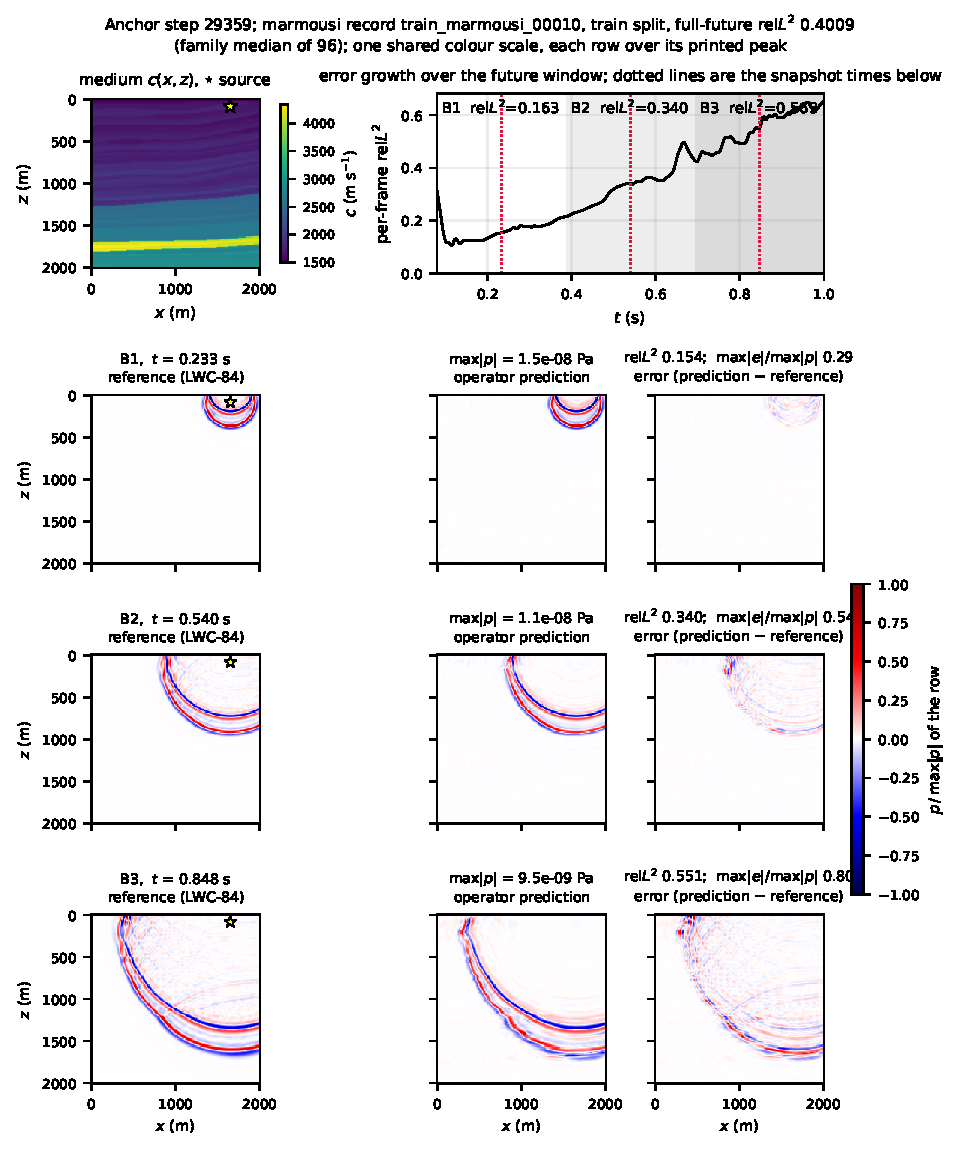
\includegraphics[width=0.99\textwidth]{fig_wavefield_snapshots_marmousi_29359.pdf}
\caption{Wavefield snapshots at the anchor, for the family-median Marmousi record
(\texttt{train\_marmousi\_00010}, full-future relative $L^2$ $0.4009$ against the family
mean $0.3965$). Top: the velocity model with the source starred, and the per-frame relative
$L^2$ over the future window, shaded by the three time bands, with the snapshot times
marked. Rows: reference LWC-84 field, operator prediction, and their difference at each
band's mid-frame. All nine panels share one dimensionless colour scale; each row is divided
by its own peak, printed on the row in Pa, so the error panel reads directly as the
fraction of the local signal the operator gets wrong ($0.29 \to 0.54 \to 0.80$). Fields are
displayed $[z,x]$ exactly as stored. Train split, checkpoint step 29359; the plotted
scores are bitwise identical to the panel rows behind Table~\ref{tab:anchor}, because the
figure imports the same measurement module at the same \texttt{sha256} rather than
reimplementing the metric.}
\label{fig:snapshots}
\end{figure}

\subsection{Error mass versus energy}

For a record with band truth energies $E_b$ and per-band relative $L^2$ values $r_b$, write
the band energy share $s_b = E_b / \sum_j E_j$. The identity
\begin{equation}
\label{eq:massid}
\mathrm{full}^2 \;=\; \sum_b s_b\, r_b^2
\end{equation}
is exact, and the \emph{error-mass share} is $m_b = s_b r_b^2 / \sum_j s_j r_j^2$. Evaluated
over all 160 anchor records, the maximum absolute residual of \eqref{eq:massid} is
$1.055\times10^{-15}$ (maximum relative residual $6.14\times10^{-15}$). The identity holds at
machine precision.

\begin{table}[t]
\centering
\caption{Energy share against error-mass share, anchor 29359, record-equal, train split.}
\label{tab:mass}
\begin{tabular}{lccc}
\toprule
Family & Energy share B1/B2/B3 & Error-mass share B1/B2/B3 \\
\midrule
uniform ($n=32$)  & $0.6793 / 0.2646 / 0.0561$ & $\mathbf{0.6055} / 0.2892 / 0.1053$ \\
layered ($n=32$)  & $0.7734 / 0.1882 / 0.0384$ & $0.2503 / \mathbf{0.4982} / 0.2515$ \\
marmousi ($n=96$) & $0.3372 / 0.3567 / 0.3061$ & $0.0672 / 0.2918 / \mathbf{0.6410}$ \\
\bottomrule
\end{tabular}
\end{table}

Three readings follow. Marmousi energy is nearly flat in time, so the late window is not a
tail of vanishing signal, yet $64.1\%$ of its error mass sits there. The families fail in
different places: uniform fails \emph{early} ($60.6\%$ of its error mass), layered in the
middle. Any intervention that trades early accuracy for late accuracy therefore damages the
family whose training-panel mean is below the $0.1$ diagnostic threshold.

An intervention confined to the early and middle windows cannot remove the observed late
error. If those windows were exact and B3 remained unchanged, each record would retain
relative error $\sqrt{s_{i,B3}}\,r_{i,B3}$. The corresponding aggregate quantities are
\begin{equation}
 r_{\mathrm{late,record}} = \frac{1}{n}\sum_i \sqrt{s_{i,B3}}\,r_{i,B3},
 \qquad
 r_{\mathrm{late,pooled}} =
 \sqrt{\frac{\sum_i N_{i,B3}}{\sum_i E_i}}.
\end{equation}
Recomputation from the stored per-record scalars gives Marmousi counterfactuals of
$0.312137$ record-equal and $0.287059$ pooled, respectively $3.12\times$ and $2.87\times$ the target.
The arithmetic and source scalars are included in \texttt{results/diagnostic\_audit\_20260922/}.
Multiplying the family-average energy share and family-average relative error would give
$0.3169$, but that operation is not an exact record-equal aggregate and is not used as a bound.
This calculation motivates reducing late error directly. It does not exclude a curriculum
or weighting change that actually improves late predictions.

Figure~\ref{fig:traces} makes the same point on a single receiver trace and adds the
cross-family contrast. Over the full future window all three predictions reproduce the
first arrival, and the uniform and layered traces are visually indistinguishable from the
reference there. The late band has to be re-normalised before it is visible at all, because
the coda sits a factor of $12.4$ (Marmousi) to $88.8$ (layered) below the first-arrival
peak; once it is, the Marmousi prediction is wrong in both amplitude and phase while the
reference is still ringing, and its B3 trace relative $L^2$ is $1.1123$ against $0.5186$
over the full window. This is the same concentration Table~\ref{tab:mass} reports as an
energy-weighted average, seen at one node.

The uniform panel of that figure is the near-zero-denominator case, and the figure labels
it as such. Its coda has left the domain through the CPML, so the re-normalisation gain is
$1.045\times10^{5}$ and the B3 trace relative $L^2$ is $156.6$ --- a division artefact of
exactly the kind \S\ref{sec:setting-metric} excludes from every claim in this paper, shown
here so that the exclusion can be checked rather than taken on trust.

\begin{figure}[!htbp]
\centering
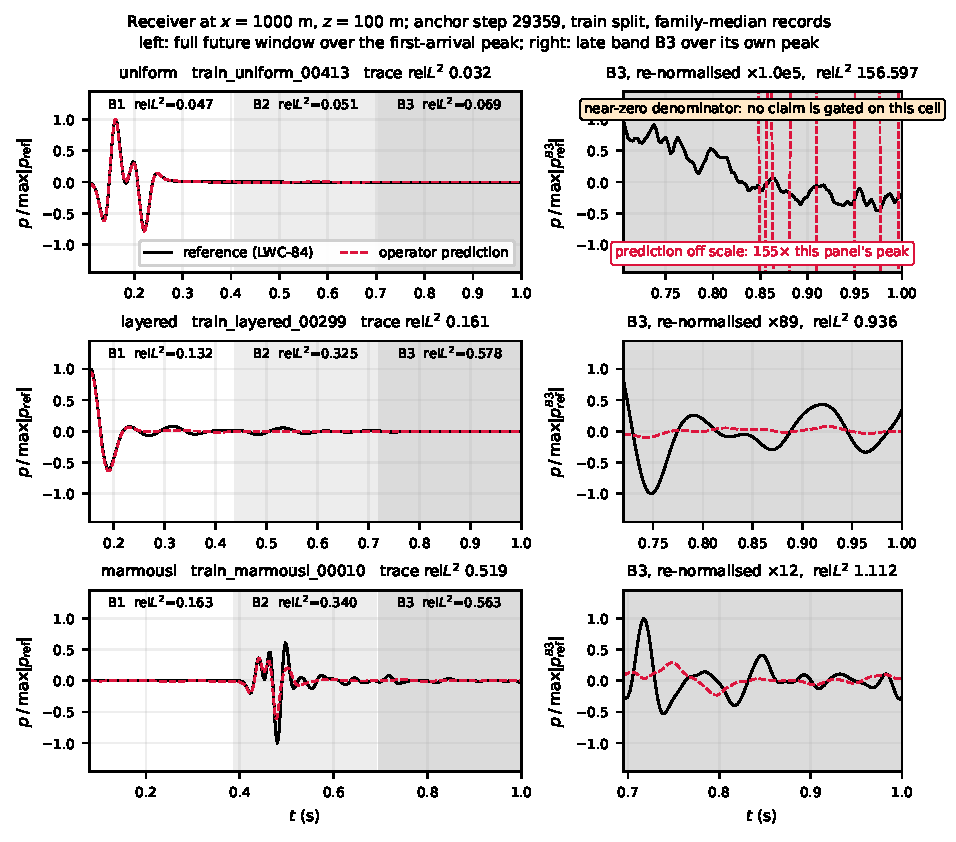
\includegraphics[width=\textwidth]{fig_receiver_traces_threefamily_29359.pdf}
\caption{Receiver waveforms at the anchor, at $x=1000$\,m and $z=100$\,m, for the
family-median record of each family. The receiver line sits $100$\,m below the surface
because the free surface is node-centred with $p(z=0)=0$ identically. Each window starts at
that record's source onset plus its 8-frame initial condition, so the three time axes begin
at different instants. Left: normalised by the reference first-arrival peak, shaded by the
three time bands with each band's field-wide relative $L^2$ printed. Right: the late band
alone, re-normalised by its own reference peak, with the gain that re-normalisation applies
stated on the panel. The uniform late panel is flagged because its denominator is near
machine zero; no claim in this paper is gated on that cell, and its prediction leaves the
re-normalised window entirely. Train split, checkpoint step 29359.}
\label{fig:traces}
\end{figure}

\section{Comparison with classical solvers and an operator baseline}
\label{sec:comparison}

This section adds three controlled comparisons: coarse-grid classical solves that exhibit
textbook numerical dispersion, receiver-level and snapshot-level views of how the neural
error differs from that dispersion, and a preregistered equal-budget DeepONet baseline.
All wavefield figures and per-record numbers in this section come from
\emph{train-development monitoring records} (the family-median records of a 9-record
dev set, 3 per family); they illustrate error character and are \emph{not} held-out
certification. The evaluated network is a subsequent lineage
(\texttt{scno\_homogeneous\_longrun\_gap15\_v1}, update 5000, $39{,}140{,}293$ parameters,
trained on a train-only frequency-gap fork of the same generation pipeline), not the
anchor of \S3; the anchor appears in this section only in the runtime rows, where it is
labelled. On the two figure records the future-window relative $L^2$ is $0.2785$
(\texttt{train\_marmousi\_00076}) and $0.1960$ (\texttt{train\_layered\_00299}), verified
by recomputation against the stored evaluation to $10^{-6}$.

\subsection{Coarse-grid classical dispersion versus the neural error}
\label{sec:comp-dispersion}

The dataset's own LWC-84 + CFS-CPML solver was re-run on coarse grids for the two figure
records, interpolated back to the stored $201\times201$ grid (bilinear, exact at shared
nodes), and scored with the paper metric. The solver requires odd node-centred grids and
raises on even $n_x/n_z$, so the nearest admissible configuration to a $50\times50$ grid
is $51\times51$ at $\Delta x=40$\,m (coarse nodes exactly on fine nodes, stride 4);
$101\times101$ at $\Delta x=20$\,m is a second point on the resolution trend. Velocities
are nodally decimated without anti-alias smoothing, so the coarse totals are
\emph{coarse-grid solution error} (time-stepping dispersion plus medium-sampling error),
both unavoidable at that resolution. Time stepping, source injection, and boundary
treatment follow the frozen native-grid benchmark protocol
(\texttt{results/paper\_comparisons\_20260923/}, group 3).

\begin{table}[t]
\centering
\caption{Coarse-grid classical solves against the neural operator, future-window relative
$L^2$ (bands B1/B2/B3 in parentheses), train-development records. The coarse columns include
medium-sampling error (see text). At $\Delta x=40$\,m the Marmousi record has $\approx3.3$
points per minimum wavelength ($v_{\min}=1500$\,m/s), below the eighth-order comfort zone;
the layered record retains $\approx4.5$ ($v_{\min}=2068$\,m/s).}
\label{tab:coarse}
\resizebox{\textwidth}{!}{\begin{tabular}{lccc}
\toprule
Record & Neural operator & LWC-84 $51\times51$ ($\Delta x=40$\,m) & LWC-84 $101\times101$ ($\Delta x=20$\,m) \\
\midrule
marmousi\_00076 & $0.279\ (0.124/0.245/0.409)$ & $0.514\ (0.470/0.514/0.558)$ & $0.120\ (0.122/0.118/0.119)$ \\
layered\_00299  & $0.196\ (0.108/0.311/0.552)$ & $\mathbf{0.103}\ (0.066/0.138/0.328)$ & $0.030\ (0.020/0.046/0.065)$ \\
\bottomrule
\end{tabular}}
\end{table}

Table~\ref{tab:coarse} and Figure~\ref{fig:comp-dispersion} show two distinct error
mechanisms. The $51\times51$ solve on the Marmousi record carries the classical dispersion
signature: receiver arrivals late by $+2.5$ to $+7.5$\,ms at three of four receivers, the
receiver spectral centroid downshifted from $12.97$ to $10.66$\,Hz, and a per-frame error
that is roughly flat in time (bands $0.470/0.514/0.558$). The neural operator error has the
opposite structure: arrivals in phase (lag $0$\,ms at most receivers; centroid $13.07$\,Hz),
but error \emph{growing} in time ($0.124 \to 0.409$ across bands) as a late-coda amplitude
deficit (receiver amplitude ratio $0.60$ at $x=400$\,m on the Marmousi record).

This dispersion argument is supported only by the Marmousi record. On the layered record
the $51\times51$ solve is \emph{more} accurate than the neural operator ($0.103$ against
$0.196$), because $v_{\min}=2068$\,m/s keeps $\approx4.5$ points per wavelength at
$\Delta x=40$\,m and its receiver lags are $0$\,ms; the $101\times101$ solve is more
accurate than the operator on both records ($0.120$ and $0.030$). We report both families;
the neural operator does not dominate coarse classical solves, and the contrast in
Figure~\ref{fig:comp-dispersion} is an error-character contrast, not an accuracy ranking.

\begin{figure}[!htbp]
\centering
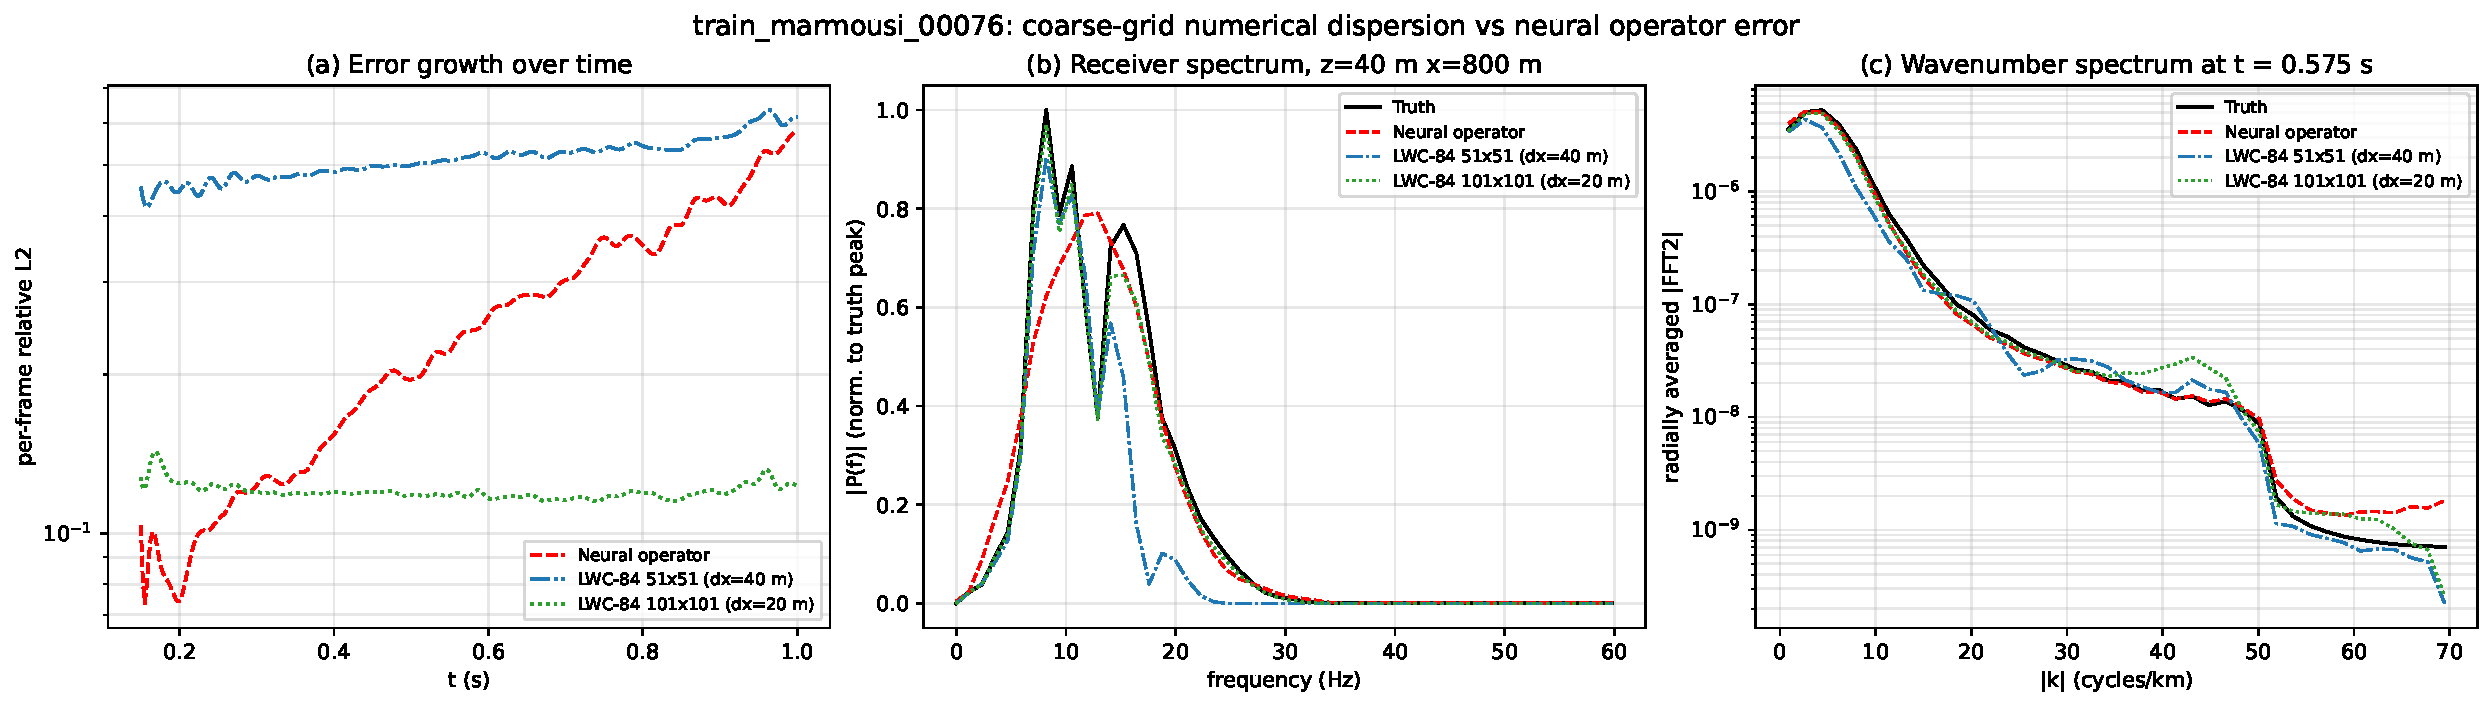
\includegraphics[width=\textwidth]{dispersion_train_marmousi_00076.pdf}
\caption{Coarse-grid numerical dispersion against neural-operator error on the
train-development Marmousi record \texttt{train\_marmousi\_00076} (not a held-out
certification).
Left: per-frame relative $L^2$ over the future window. Middle: receiver amplitude spectrum
at $z=40$\,m, $x=800$\,m; the $51\times51$ solve loses the band above $\approx15$\,Hz
(centroid $12.97 \to 10.66$\,Hz) while the neural trace keeps the truth band. Right:
radially averaged wavenumber spectrum at $t=0.575$\,s. Fields are $[z,x]$ as stored.}
\label{fig:comp-dispersion}
\end{figure}

\subsection{Snapshots and receiver waveforms}
\label{sec:comp-fields}

Figures~\ref{fig:comp-snap-marmousi} and~\ref{fig:comp-snap-layered} show truth,
prediction, and difference at early/middle/late physical times for the two records.
Both records reproduce the direct wavefront and lose scattered coda with time: per-frame
relative $L^2$ grows from $0.094$ ($t=0.2175$\,s) to $0.242$ ($t=0.575$\,s) to $0.580$
($t=1.0$\,s) on the Marmousi record, and from $0.045$ to $0.318$ to $1.010$ on the layered
record, whose final stored frame is at the trivial-predictor level while its full-window
score remains $0.1960$. This is the same late-time structure as the anchor diagnosis of
\S3, on a different lineage.

Figure~\ref{fig:comp-receivers} overlays the $51\times51$ coarse solve on the receiver
waveforms. The coarse trace arrives late and rings (dispersive tail); the neural trace
stays in phase through the first arrivals and then loses late-coda amplitude. The receiver
nodes at $x\in\{400,800,1200,1600\}$\,m, $z=40$\,m are native coarse nodes (stride-4
multiples), so the plotted coarse traces are solver values, not interpolants.

\begin{figure}[!htbp]
\centering
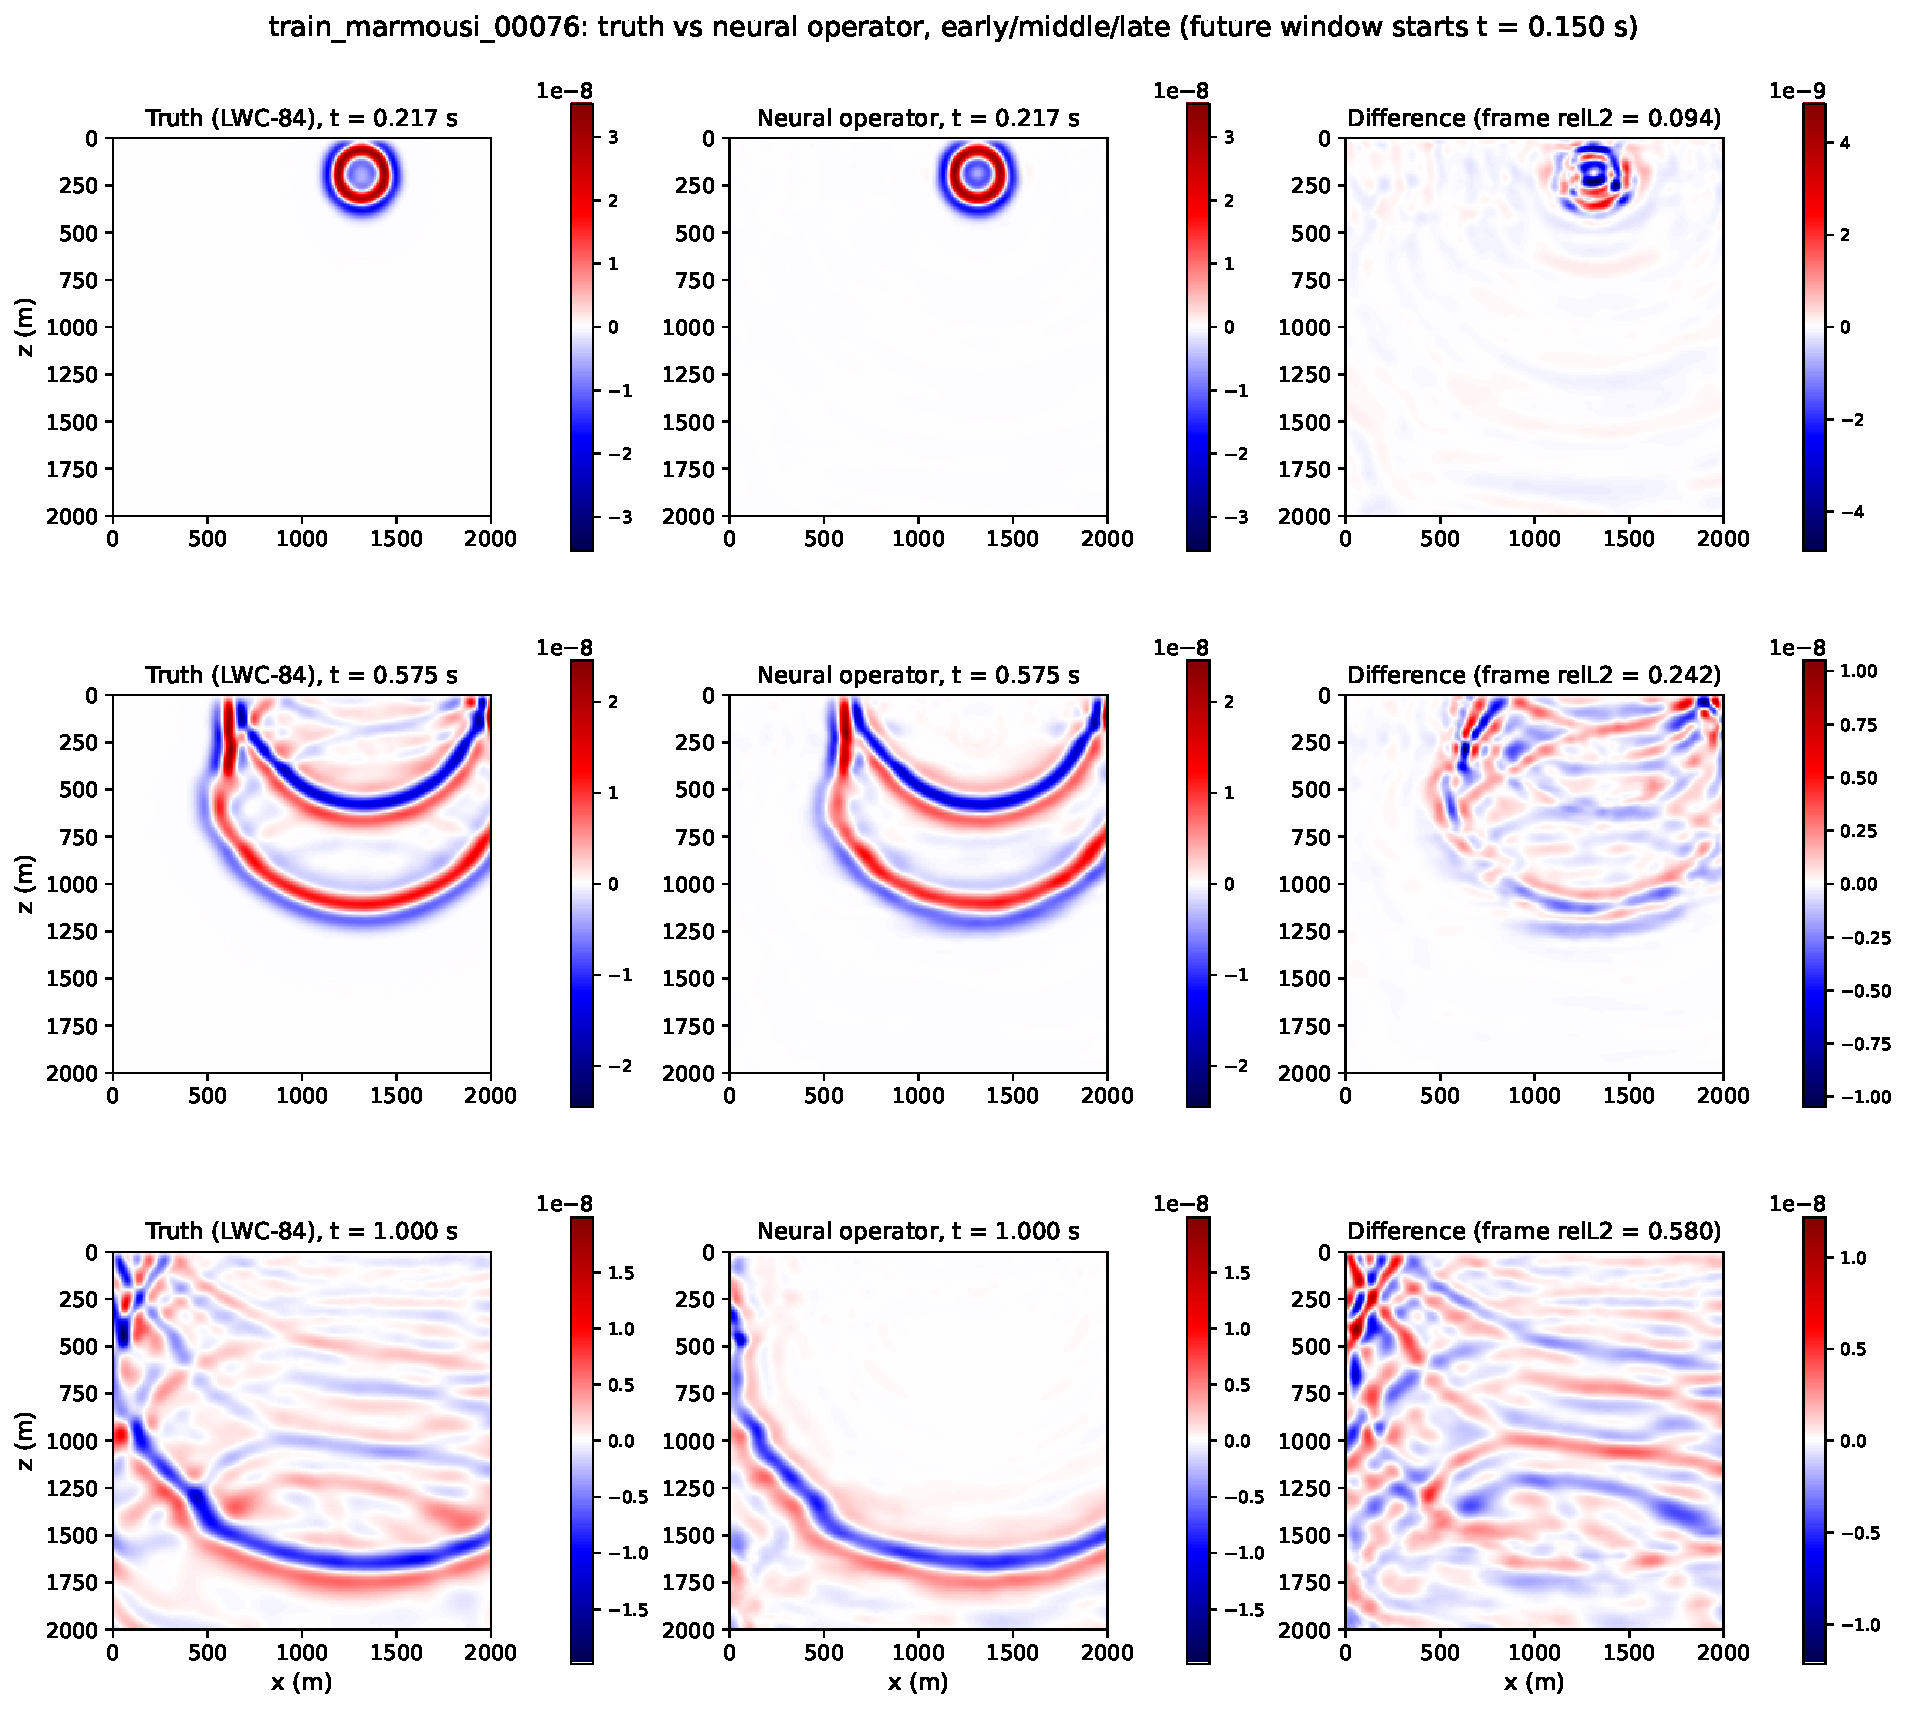
\includegraphics[width=0.94\textwidth]{snapshots_train_marmousi_00076.pdf}
\caption{Truth, neural prediction, and difference at early/middle/late times on the
train-development Marmousi record \texttt{train\_marmousi\_00076} (not held-out
certification).
Truth and prediction share one symmetric colour scale per row; the difference column has
its own symmetric scale per row. Per-frame relative $L^2$ is printed on each difference
panel. Fields are displayed $[z,x]$ exactly as stored, depth increasing downward.}
\label{fig:comp-snap-marmousi}
\end{figure}

\begin{figure}[!htbp]
\centering
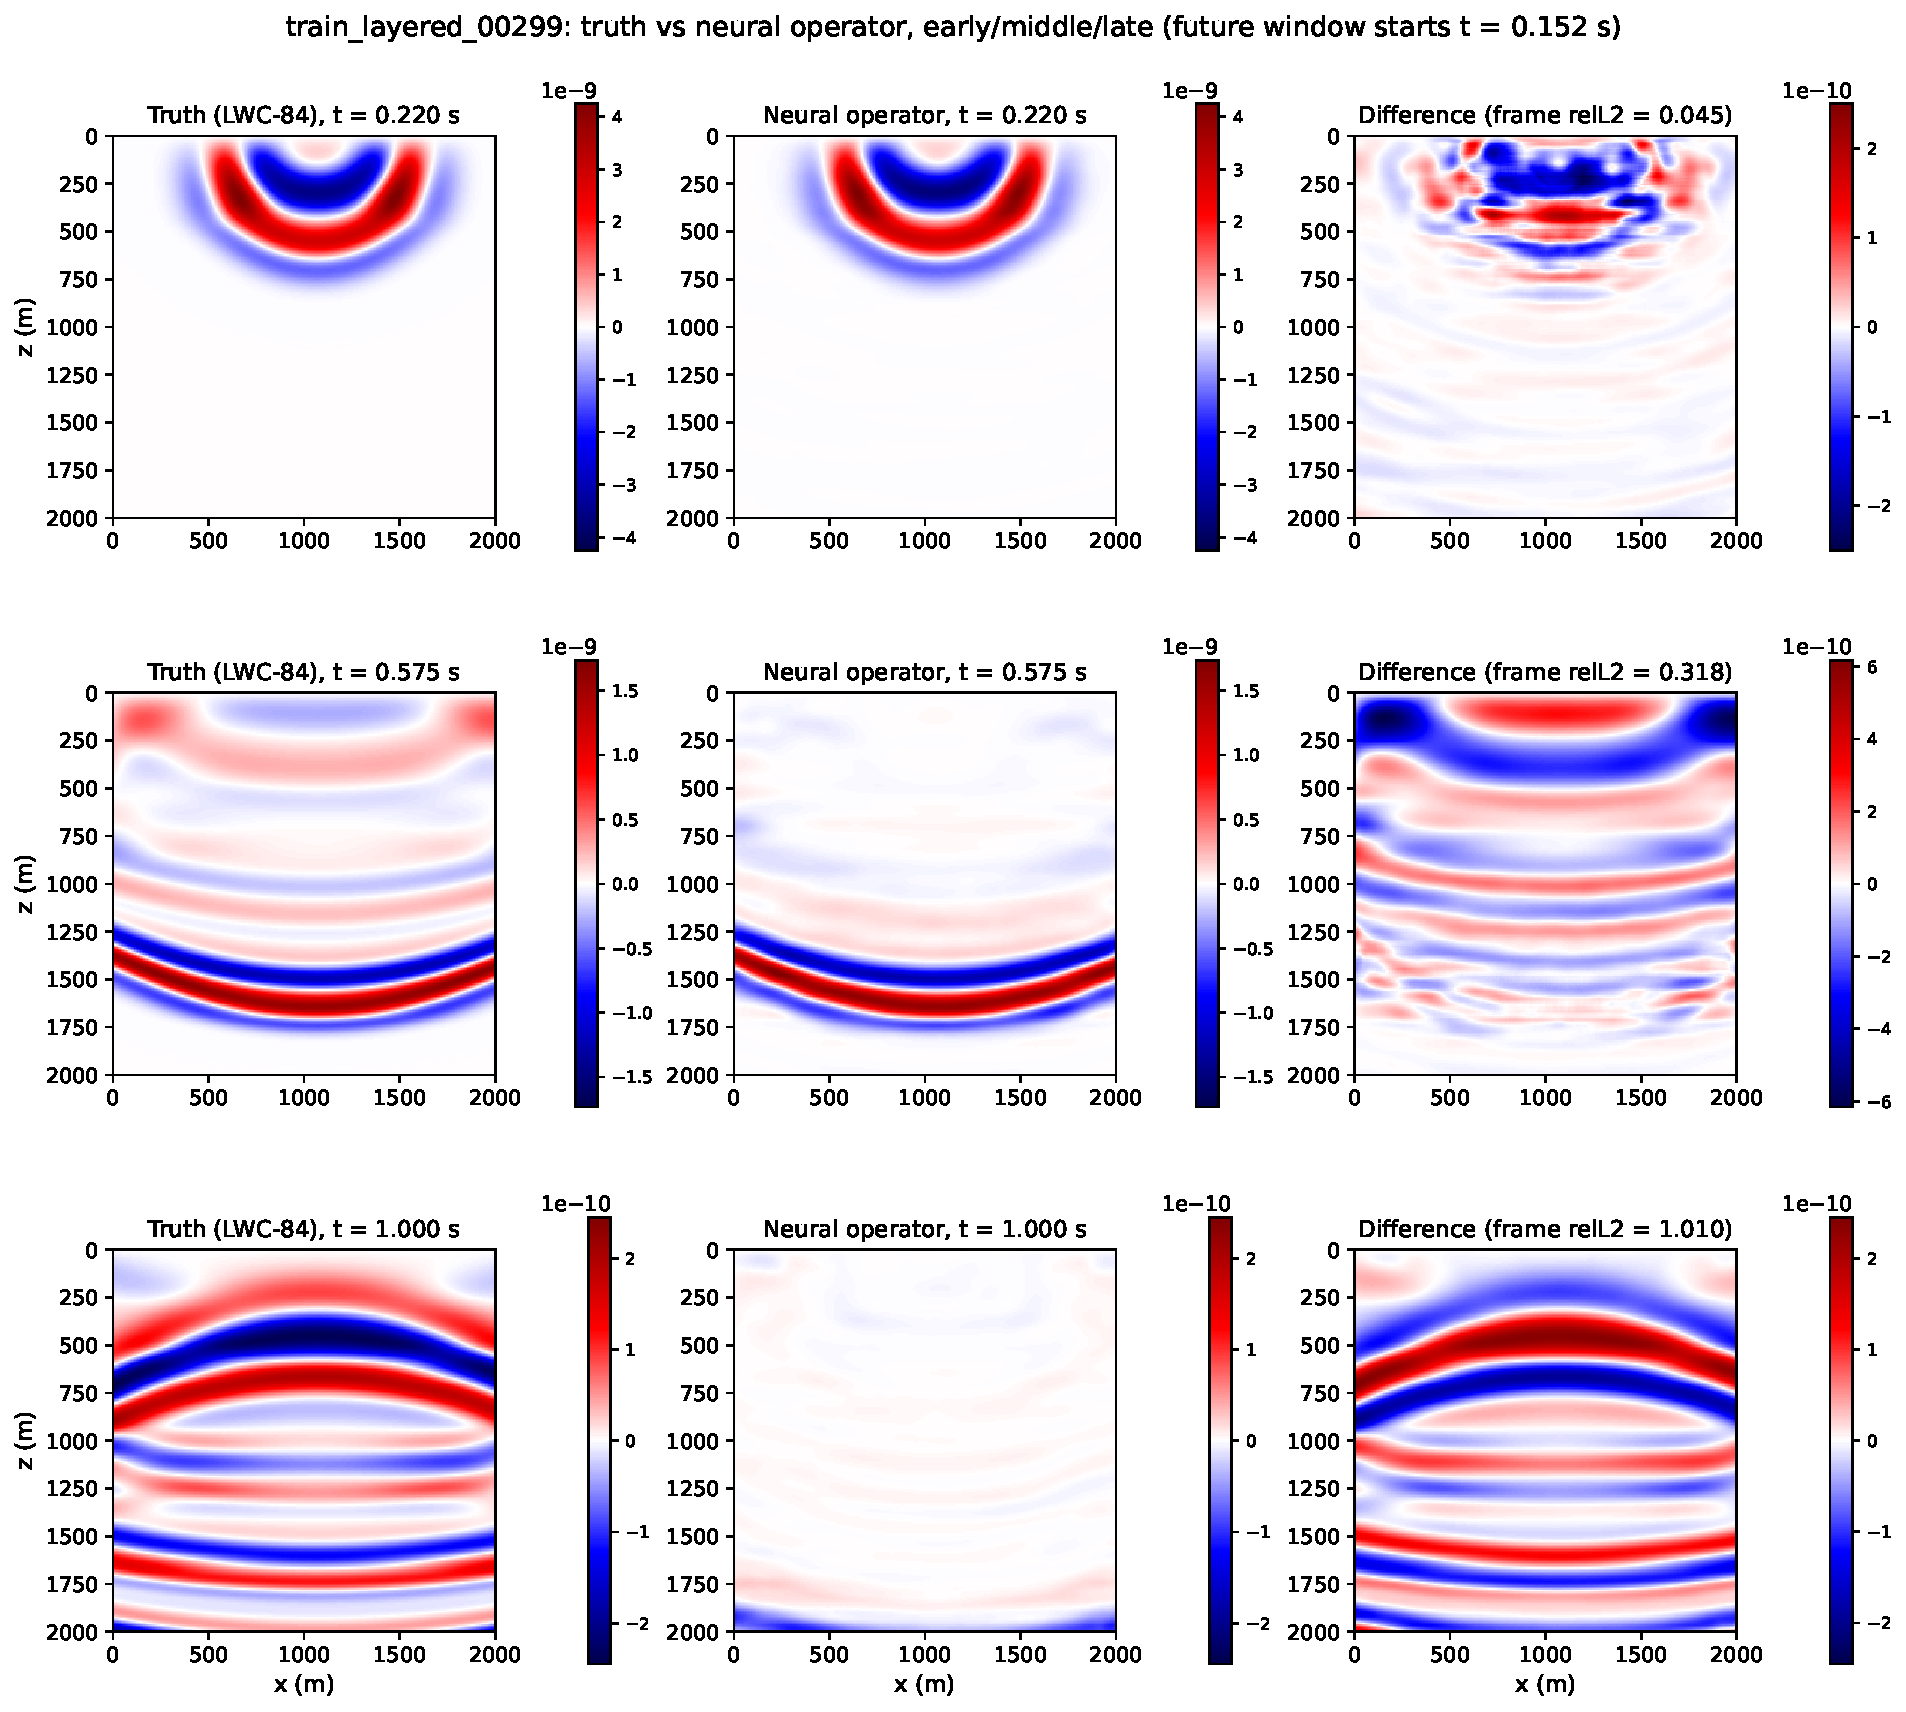
\includegraphics[width=0.94\textwidth]{snapshots_train_layered_00299.pdf}
\caption{As Figure~\ref{fig:comp-snap-marmousi}, for \texttt{train\_layered\_00299}
(train-development record; not held-out certification). The final stored frame reaches
per-frame relative $L^2$ $1.010$: the prediction retains almost none of the reverberating
coda at $t=1.0$\,s, although the full-window score is $0.1960$.}
\label{fig:comp-snap-layered}
\end{figure}

\begin{figure}[!htbp]
\centering
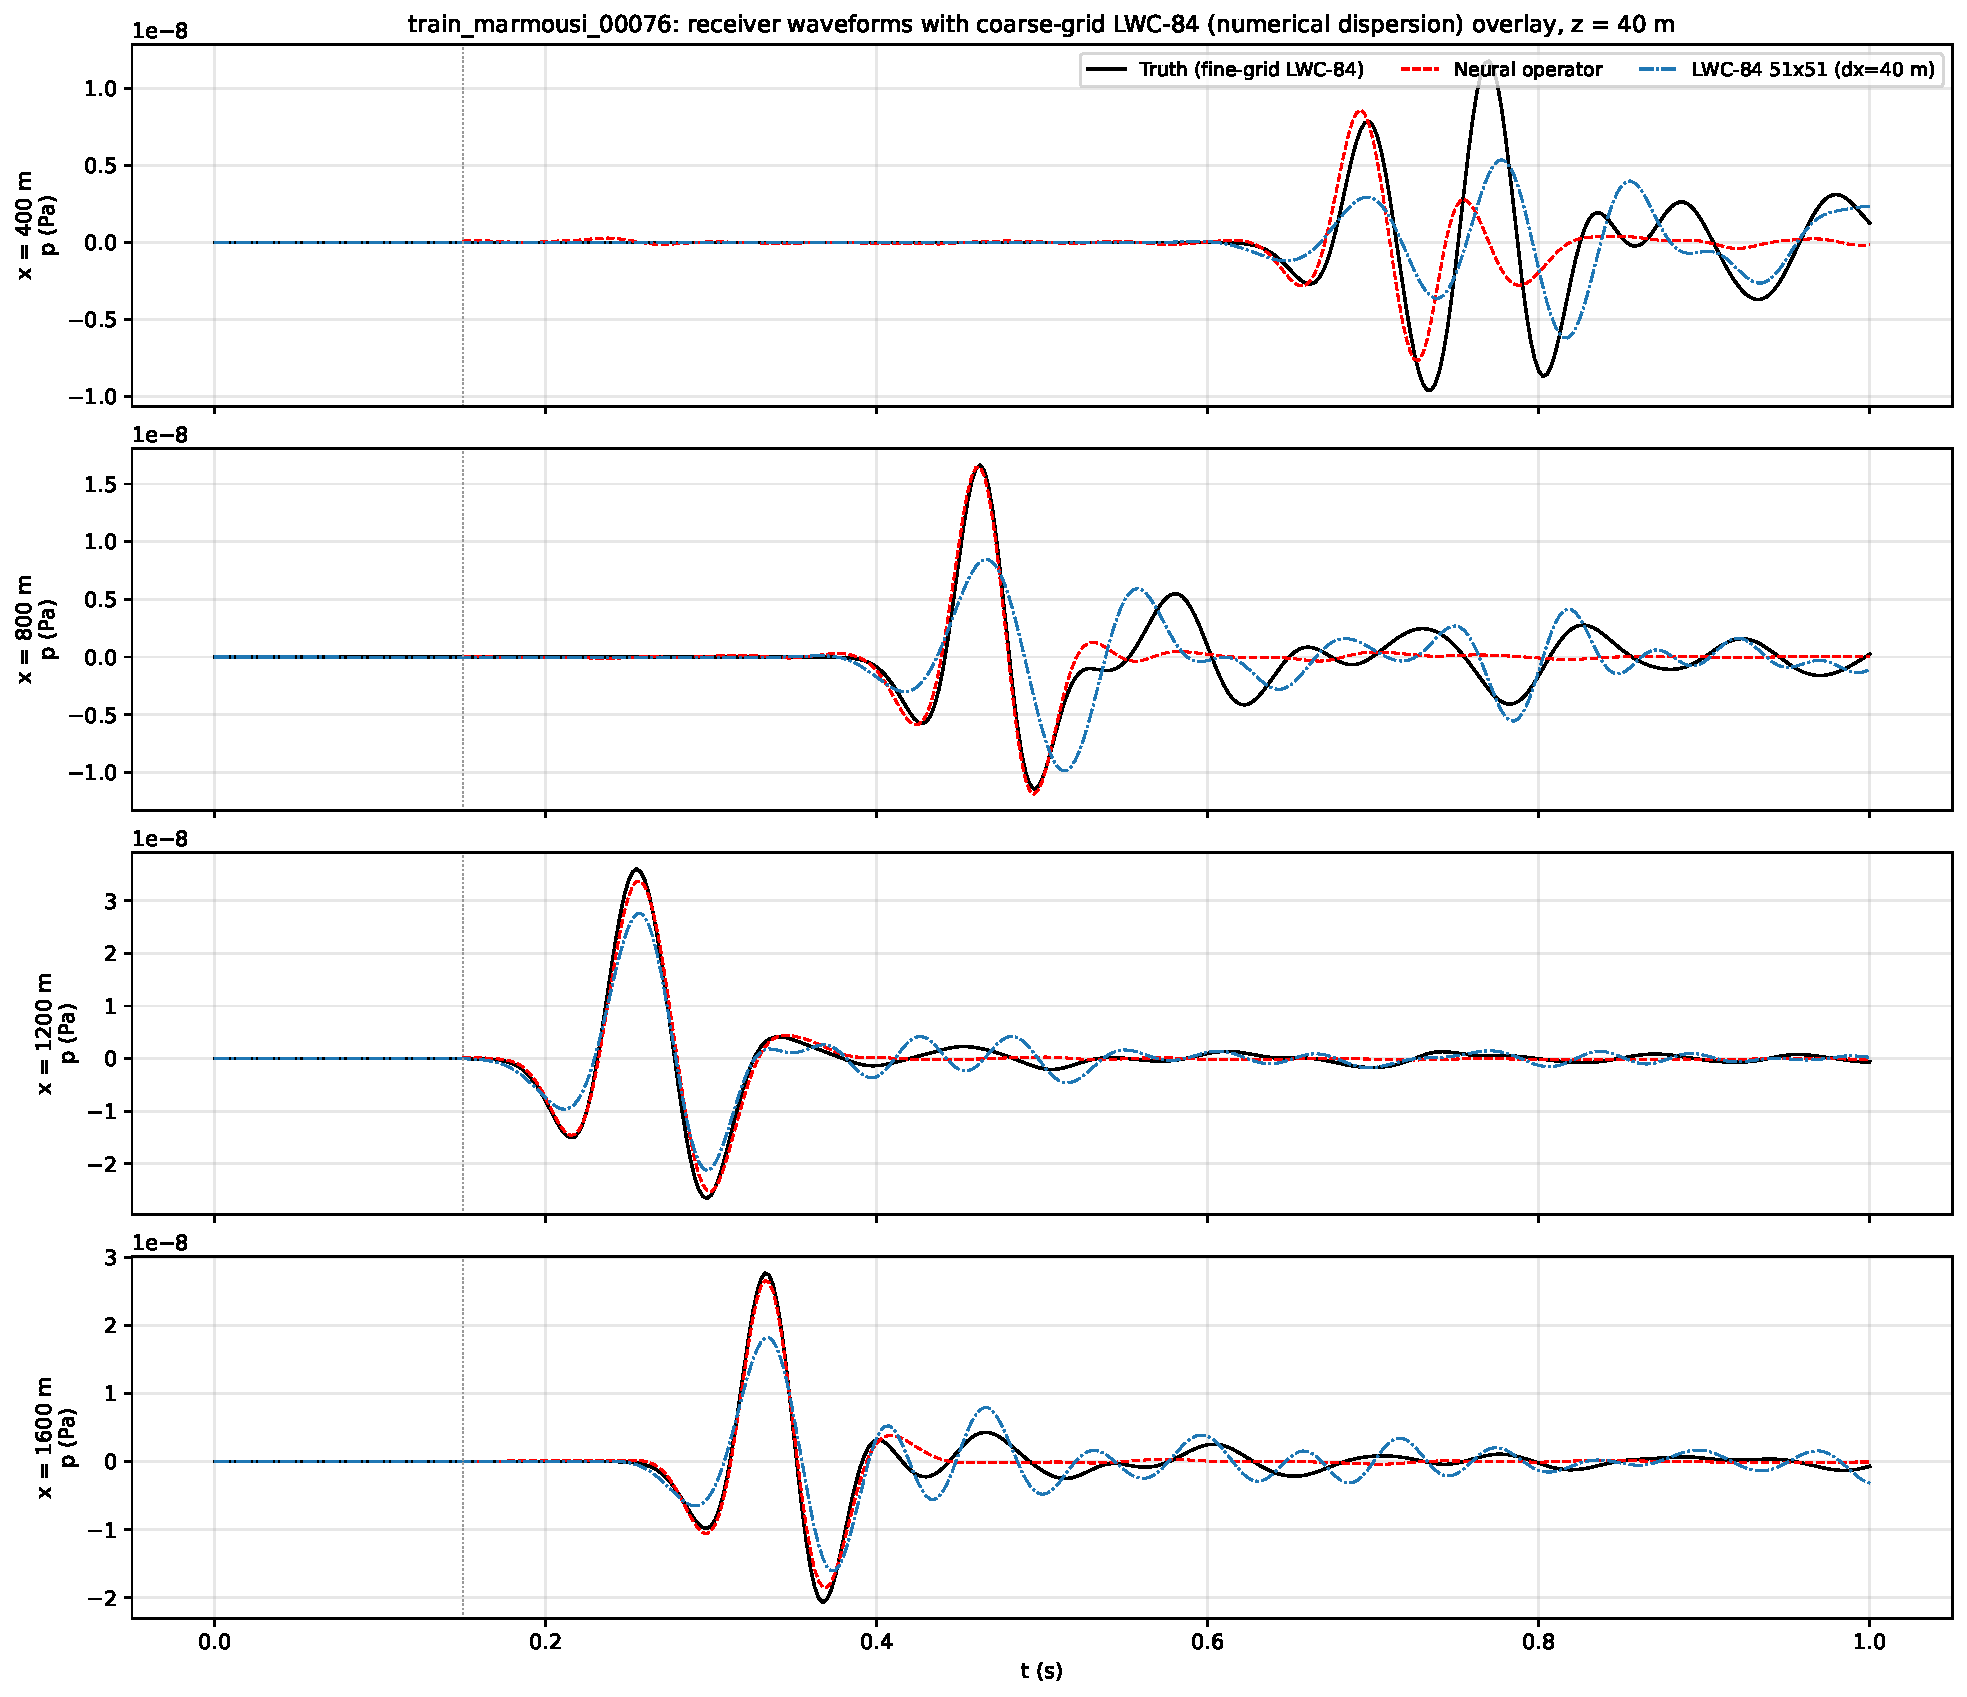
\includegraphics[width=\textwidth]{receivers_dispersion_train_marmousi_00076.pdf}
\caption{Receiver waveforms at $z=40$\,m for \texttt{train\_marmousi\_00076}
(train-development record; not held-out certification): truth, neural operator, and the
$51\times51$ coarse LWC-84 solve. The coarse trace shows phase lag and ringing (numerical
dispersion); the neural trace is in phase but under-predicts the late coda. The dotted
line marks the start of the future window.}
\label{fig:comp-receivers}
\end{figure}

\subsection{Runtime in context}
\label{sec:comp-runtime}

The timing protocol and numbers are those of \S\ref{sec:runtime}
(Table~\ref{tab:runtime}); no new timing runs were performed. Assembled record-matched
ratios: the anchor operator is $5.06\times$ (standard) and $7.90\times$ (16-frame batched)
faster than the fine-grid protocol, and $2.52\times$/$3.93\times$ faster than the native
$201\times201$ solve; the independent generation-protocol timing on validation records is
$22.06$\,s. Two caveats bound any speed claim. First, the cheapest tested classical
configuration (native grid, $10.00$\,s) is more accurate than the anchor operator on every
family-median record in Table~\ref{tab:runtime}, so the
speed advantage carries an accuracy cost on every family. Second, training is amortised
and excluded; no end-to-end (training-inclusive) speedup is claimed.

\subsection{An equal-budget DeepONet baseline failed to train}
\label{sec:comp-deeponet}

A preregistered DeepONet baseline at matched parameter budget ($39{,}975{,}985$ against
our $40{,}484{,}837$; budget $\pm2\%$; the reference is the IC8 40-M configuration behind
the A4 lineage, not the $39.1$-M anchor of \S2) was trained on the same task. Its main run was
terminated by SIGTERM at step $4{,}862$ of a planned $22{,}814$, so its numbers are not a
converged endpoint. At every recorded validation on its fixed 12-record checkpoint-selection
batch, its dense relative $L^2$ was $1.000012$--$1.000014$, indistinguishable from the
trivial zero predictor on all three families. A subsequent family-level probe (12 train
records, 2000 steps) found the control arm never below $1.0015$, and an anti-collapse arm
oscillating at $0.97$--$1.33$, not separable from control on any of its three effect axes;
single-record fits do converge (relative $L^2$ $0.025$ at 2000 steps), so the recorded
verdict attributes the failure to optimisation, not capacity.

\begin{table}[t]
\centering
\caption{DeepONet baseline at matched parameter budget. No same-caliber comparison exists:
the DeepONet run stopped early and was never evaluated on the 480-record census, so the
rows pair the nearest available calibers and each row names its own. The comparison
establishes that this baseline failed to train in this setting; it is not an accuracy
ranking between converged models.}
\label{tab:deeponet}
\resizebox{\textwidth}{!}{\begin{tabular}{lccl}
\toprule
Quantity & DeepONet 40M & Ours (IC8 40M) & Caliber \\
\midrule
Parameters & $39{,}975{,}985$ & $40{,}484{,}837$ & same $\pm2\%$ budget (preregistered) \\
Fixed 12-record validation, dense rel.\ $L^2$ (best, step 4488) & $1.000012$ & n/a (not our selection metric) & DeepONet's selection batch; $\approx1.0$ = trivial \\
480-record validation census, dense future rel.\ $L^2$ & not evaluated (stopped at step 4862/22814) & $0.352$ ($0.131/0.302/0.565$) & ours: full census, A4 step 22814 \\
12-record family probe (2000 steps), point rel.\ $L^2$ & control $1.0015$--$1.1168$, never $<1.0$ & n/a & packaged-loss probe caliber \\
\bottomrule
\end{tabular}}
\end{table}

Table~\ref{tab:deeponet} states the recorded facts. Because the baseline collapsed, these
numbers support only the statement that \emph{this DeepONet configuration failed to train
in this setting under its preregistered protocol}; they do not support a claim that our
operator outperforms a converged DeepONet, and we make no such claim.

\section{Intervention tests and their scope}

Table~\ref{tab:elim} summarizes the tested alternatives. Frozen protocols accompany the
major intervention arms. Each result constrains the specified implementation, data panel,
and budget; it does not exclude the broader method class.

\begin{table}[t]
\centering
\caption{Diagnostic tests and their scope. Negative findings apply to the tested settings.}
\label{tab:elim}
\begin{tabular}{p{0.28\textwidth}p{0.62\textwidth}}
\toprule
Candidate & Measurement and interpretation \\
\midrule
Spectral truncation bandwidth &
Truth energy outside the anchor's radial-44 kernel is $0.882\%$; zeroing \emph{all}
out-of-band error buys at most $1.02\times$ ($1.27\times$ at rect16) against $4.05\times$
needed. \\
The error is high-wavenumber &
Band-3 truth is \emph{narrower} than band-1 ($10.85\%$ against $14.71\%$ outside rect16)
while its error is $2.4\times$ larger. \\
Width / capacity &
An internal width sweep saturates near $0.125$; this does not exclude different capacity allocation or architectures. \\
Optimiser / gradient clipping &
Releasing the clip is $+135.8\%$ (clip $=20$) and $+163.8\%$ (clip $=10^9$), worse on
$44/44$ paired steps. Steps are serially dependent, so this is a descriptive comparison. \\
Inference-time iteration of the trained correction &
$n=2$ is $+1.21\%$ ($19/20$ worse); $n=3$ is $+3.69\%$ ($20/20$ worse). \\
One proposed reflection carrier &
The strongest-impedance single bounce arrives at $1.62$--$1.75$\,s, outside the $1.0$\,s
record. This excludes that path as an in-window carrier, not other scattering paths. \\
A bad tail of records &
Forcing the worst $30\%$ to $0.1$ reaches only $0.2698$; putting \emph{every} record at the
current $p_{10}$ reaches only $0.2657$. \\
Sampling energy-floor artefact &
The floor fires on $0.0\%$ of Marmousi frames (uniform $23.43\%$, layered $2.02\%$). \\
Frame re-weighting &
The weighted mean is invariant to $w \to c\,w$, so ``down-weight early'' and ``up-weight
late'' are equivalent only when their normalized relative weights are identical; general re-weighting remains open. \\
\bottomrule
\end{tabular}
\end{table}

\paragraph{The deployed discrete residual changes the supervised norm.}
The source-aware LWC-84 increment term was enabled at weight $0.01$ in 37 production runs,
including the anchor lineage. Its weighted objective share is $0.0038\%$--$0.18\%$.
This is a small value contribution, although loss magnitude alone does not determine its
gradient contribution.

For the deployed defect-matched form, the linear increment operator $A$ gives
$A(\mathrm{pred})-A(\mathrm{label})=A(\mathrm{pred}-\mathrm{label})$.
The audit confirms this identity over 288 triplets, with maximum relative deviation
$4.57\times10^{-13}$. The term therefore provides a physics-derived weighting of supervised
error, rather than an independent equation constraint at unlabeled times. Such weighting may
still improve optimization or accuracy; the identity does not prove that increasing its weight
cannot help.

Its weighting differs substantially from the field-error distribution. In a six-band audit,
$79.9\%$ of error energy lies in the smoothest band, compared with $27.3\%$ of $\lVert Ae\rVert^2$.
The penalty amplifies high-wavenumber errors, and its framewise rank correlation with relative
$L^2$ changes sign across families. These observations motivate gradient and transfer checks
before changing its weight. They do not establish the outcome of an unrun weight sweep.

A label-free residual needs a discretization consistent with the stored product. Labels are
lowpass restrictions of a finer solve, and their own late Marmousi defect is $1.069\%$ under
the audited operator. Stored cadence is $2.5$\,ms on $10$\,m spacing, versus $0.125$\,ms on
$5$\,m spacing during generation. At $7963$\,m/s these imply Courant numbers of $1.99$ and
$0.199$. A large-step increment residual need not approximate the generator accurately;
this is not by itself a statement about neural-network stability. The radius-20 interior
margin also excludes roughly $36\%$ of the stored area. Free-surface extensions and CPML
memory states require explicit treatment. We therefore leave weak-form, substepped, and
boundary-aware residuals as distinct experiments.

\subsection{The counter-experiment}

To test whether releasing the collapsed correction branch and switching to a phase-free
rectangular spectral kernel breaks the floor, an 18700-step arm was run from the anchor to
step 48059 under a frozen pre-registration. Table~\ref{tab:armr4} gives the result: the main
gate required $\mathrm{B3}(M96) \le 0.5441354$ and measured $0.5889980$. Every family got
worse. Run integrity was clean: 18700 contiguous steps, zero duplicates, zero rejected
retries, zero non-finite events.

\begin{table}[t]
\centering
\caption{Counter-experiment arm at step 48059 against the anchor, record-equal, train split.}
\label{tab:armr4}
\begin{tabular}{lrrr}
\toprule
Cell & Anchor & Arm & $\Delta$ relative \\
\midrule
Marmousi B3 (main gate, $n=96$) & $0.572774$ & $0.588998$ & $+2.83\%$ \\
Marmousi full ($n=96$)          & $0.396499$ & $0.423210$ & $+6.74\%$ \\
layered full ($n=32$)           & $0.230264$ & $0.258124$ & $+12.10\%$ \\
uniform full ($n=32$)           & $0.060902$ & $0.116177$ & $+90.76\%$ \\
\bottomrule
\end{tabular}
\end{table}

Training loss fell by roughly $6\%$ over the window, the only one of four arms to leave its
plateau, while error on the frozen training-panel evaluation rose in every family. The per-record paired damage
fits the descriptive relationship $b=\sqrt{a^2+c^2}$. The fitted $c$ values are
$0.09846$, $0.11119$, and $0.14661$ for uniform, layered, and Marmousi, respectively.
The corresponding $R^2$ values are $-0.460$, $0.9560$, and $0.9417$.
Record ranking is largely preserved (Spearman $0.978$ and $0.969$ on layered and Marmousi). This fit describes the paired scores for layered and Marmousi records. It is consistent
with an added error component, but scalar error norms do not establish vector orthogonality
or identify its cause. Several settings changed together, so the arm cannot isolate kernel
shape from gating or supervision effects. The uniform fit is poor ($R^2<0$).

\section{Temporal-transfer and correction diagnostics}

\subsection{Limited transfer between supervised and unsupervised frames}

In a single-record adaptation probe with 16 supervised frames, relative $L^2$ on a disjoint
16-frame late set changes from $0.37067$ to $0.36479$, a ratio of $0.9841$.
The temporal offsets are only $2.5$--$17.5$\,ms. Increasing supervision to 51 frames gives
$0.19163$, a ratio of $0.5170$ to the same initial error. It also increases the number of
evaluation frames within $10$\,ms of a supervised frame from 0 to 11 out of 16.

The deployed supervision spacing is a mean gap of $56.78$\,ms with \emph{no} gap below
$10$\,ms, while the truth's own correlation drops below $0.5$ between $10$ and $20$\,ms. The
probe therefore requires interpolation across gaps wider than the measured decorrelation
scale. Its limited transfer is consistent with frame-specific adaptation. The 51-frame probe
demonstrates a within-record density effect, but not cross-medium generalization or a
validation-wide accuracy improvement.

\subsection{Scale collapse of the correction branch}
\label{sec:orth}

The decoder forms $y_d=c+s\,r$, followed by the fixed free-surface factor
$F(z)=\tanh^2(z/(20\,\mathrm{m}))$. The deployed prediction is therefore $F(c+s\,r)$.
Define the deployed baseline error $e=Fc-y_{\mathrm{truth}}$ and correction $q=Fr$.
For fixed nonzero $e$ and $q$, least squares gives
\begin{equation}
\label{eq:orth}
\min_g \frac{\lVert e+gq\rVert}{\lVert e\rVert}
=\sqrt{1-\cos^2(q,-e)},\qquad
 g^\star=\frac{\langle-e,q\rangle}{\lVert q\rVert^2}.
\end{equation}
This identity bounds rescaling of a fixed correction direction. It does not bound a branch
whose features are retrained.

A forward-only audit captures the pre-gate correction directly and evaluates 144 frames
from 12 training records. The median optimal ratio in deployed output space is $0.999234$,
a $0.0766\%$ median reduction relative to the coarse-only error. This oracle fits an independent
scalar to each frame using its true residual. It is consequently more permissive than a
single deployable gain, and is not a family-level accuracy score. The recorded reconstruction
check has maximum relative error $1.03\times10^{-15}$, with weights unchanged bitwise.

An earlier probe omitted $F$ from the compared decoder tensors and reported $0.9984$.
That decoder-space number is superseded for deployment interpretation. The corrected audit
and its script are included in \texttt{results/diagnostic\_audit\_20260922/}.
The anchor gate remains $s=1.0425\times10^{-4}$; neither its size nor the oracle proves that
training found a globally optimal decomposition. The result shows limited improvement from
rescaling the current direction and motivates learning a different direction.

\paragraph{Gate-dependent gradients motivate a different training target.}
A frozen-output scale sweep measures log-log gradient slopes near one for several correction
modules: $1.041$ for the output weight and $1.007$ for the dense spectral kernels. Parameters
outside the dense decoder have a near-zero slope. This agrees with the chain-rule factor
$s$ in $\partial L/\partial W_r$. The measured objective increases when the current frozen
branch is opened, including $+129.8\%$ at $s=1$. These measurements explain why opening this
trained gate alone is unpromising; they do not prove that joint retraining has the same optimum.

Directly supervising the deployed correction $q=Fr$ against the detached target
$y_{\mathrm{truth}}-Fc$ would provide a branch gradient without that multiplicative gate. A frozen-feature least-squares probe
reports a transferable ratio of $0.9998$, so any improvement would require learning new
features. Changes to attention, local convolutions, initialization, or staged optimization
remain untested. Sharing a scalar gate does not prove that another architecture must learn
the same correction direction.

\section{Frequency-resolved error and conditional improvement estimates}

Using the frequency-resolved error decomposition over the 480-record validation evaluation
(four radial wavenumber bands, Parseval verified per frame), band relative $L^2$ rises
monotonically with wavenumber: $0.3641 / 0.5263 / 0.7566 / 0.9924$ pooled. Independently, the
prediction carries \emph{less} above-mode-16 energy than the truth in all three families
($0.1669$ against $0.1871$ for uniform, $0.0465$ against $0.0598$ for layered, $0.2100$
against $0.2299$ for marmousi). Together these indicate an endpoint frequency-dependent error pattern. Learning dynamics
would be needed to establish when each frequency is learned.

We use two counterfactuals to quantify the error remaining under restricted changes. One
sets bands 3 and 4 to zero error while preserving lower bands. The other gives every band
the current lowest-band relative error. Because $\sum_b s_b=1$, this second score equals
the current lowest-band value. Neither counterfactual is a demonstrated intervention or an
upper bound on methods that also reduce low-band error. Table~\ref{tab:ceil} reports both.

\begin{table}[t]
\centering
\caption{Conditional spectral counterfactuals, A4 step 22814, validation split, 480 records.}
\label{tab:ceil}
\begin{tabular}{lrrrrr}
\toprule
Family & $n$ & pooled & bands 3+4 $\to 0$ & fully flattened & gap to $0.1$ \\
\midrule
uniform  & 90  & $0.17276$ & $0.1557\ (-9.9\%)$ & $0.1114\ (-35.5\%)$ & $1.11\times$ \\
layered  & 240 & $0.28986$ & $0.2827\ (-2.5\%)$ & $0.2369\ (-18.3\%)$ & $2.37\times$ \\
marmousi & 150 & $0.50382$ & $0.4779\ (-5.1\%)$ & $0.3980\ (-21.0\%)$ & $\mathbf{3.98\times}$ \\
pooled   & 480 & $0.47588$ & $0.4514\ (-5.1\%)$ & $0.3641\ (-23.5\%)$ & $3.64\times$ \\
\bottomrule
\end{tabular}
\end{table}

Most error mass lies in band 2 ($64.7\%$ pooled), with only $0.5\%$ in the highest band.
Eliminating bands 3 and 4 alone reduces pooled error by $5.1\%$. Marmousi has the smallest
relative enrichment of error in band 3 among the three families: its
band-3 error enrichment is $2.309$ against $8.690$ and $9.467$ for uniform and layered, and
its truth is the widest-band of the three. Its substantial low- and middle-band errors motivate interventions beyond the spectral tail.
This endpoint comparison does not exclude dynamical spectral bias.

Marmousi band 4 has relative $L^2$ of $1.0412$, and uniform band 4 falls below band 3.
Both bands contain only about $0.1\%$ of total truth energy and contribute little to the
pooled score. Small relative energy alone does not establish a numerically ill-conditioned
denominator; that interpretation requires absolute-energy and noise-floor checks.

\section{Related work}

\paragraph{Learned background and correction branches have precedent.}
Balaji et al.~\cite{highcontrast} combine an FNO background with a transformer correction for
high-contrast Helmholtz scattering. We make no novelty claim for a two-branch decomposition.
Their frequency-domain setting, architecture, and training differ from our time-domain
full-wavefield task. Their reported success establishes a relevant precedent, but does not
isolate attention as the cause of improved accuracy. Our contribution is the diagnostic
analysis of one trained implementation and the scope of its failed interventions.

\paragraph{Frequency diagnostics connect to rollout research.}
\cite{pderefiner} identifies the neglect of non-dominant spatial frequency information, often
high frequencies, as the primary pitfall limiting stable accurate rollouts. Our measurement
that the prediction carries less above-mode-16 energy than the truth in all three families is
a related endpoint observation in a single-shot setting, without testing the same rollout
mechanism. \cite{spectralbias} argues that spectral bias in operator learning is dynamical rather
than purely representational and recommends curvature-aware optimisation and spectrally
informed losses; both are untested here (\S\ref{sec:limits}).

\paragraph{Structured spectral rollout methods do not transfer directly.}
\cite{sgno} reports large long-horizon gains for a structured spectral autoregressive operator,
but states that it is designed for periodic linear and semilinear evolution PDEs with Fourier
multiplier linear dynamics. Our problem is variable-coefficient, with CPML absorbing boundaries
and a free surface, and is neither periodic nor a Fourier multiplier. We cite the method for
its diagnosis of spectral amplitude and phase drift, and we do not transfer its reported
factors to our setting.

\paragraph{Learned dispersion correction: the nearest precedent is fixed-velocity.}
\cite{nnaugmented} treats an inaccurate finite-difference Laplacian as incomplete physics and
intersperses CNNs between low-fidelity timesteps to limit numerical dispersion during
propagation. It is a proof of concept that holds the velocity model fixed and varies only
source locations. \cite{dispersion} benchmarks twelve correction architectures for 2-D
anisotropic acoustic dispersion over 27{,}000 heterogeneous velocity fields, finding the FNO
best but by a modest margin over a CNN, and finding that pipelines with a classical initial
guess substantially outperform those learning the correction directly; it operates on traces
rather than full wavefields. Coarse-grid-plus-learning accounting in other domains closes
favourably. \cite{barsinai} integrates 1-D equations at 4--8$\times$ coarser resolution and
\cite{kochkov} matches baseline solvers at 8--10$\times$ finer resolution for 2-D turbulence,
a 40--80$\times$ net speedup with stability over long simulations. The former is 1-D and
the latter is Navier--Stokes, a first-order-in-time advection-dominated system, so neither
transfers to a second-order hyperbolic problem without demonstration.

\section{Limitations}
\label{sec:limits}

\paragraph{Split leakage is disclosed.} The Marmousi family contains 50\,m-stride translated
twins, with 30 of 30 audited models having a twin. Marmousi numbers on held-out records are
therefore \emph{not} clean generalisation measurements.

\paragraph{Lineage.} The band decomposition is the validation split at a radial-44 endpoint
with 16-frame supervision. The counter-experiment arm is rectangular-kernel with 16 frames.
The subsequent density arm uses 51 frames and is a separate experiment.
The dense spectral kernel sets the wavenumber response, so the band table does not
characterise the rectangular-kernel lineage, and no frequency-resolved product exists for that
lineage on either split.

\paragraph{Learning dynamics are not measured.} Whether high-wavenumber bands converge later
than low ones is not answered here. This distinction separates learning dynamics from
endpoint representational error. The frequency-resolved metric is driven by offline
evaluation, which was run at a single endpoint; answering it requires evaluation at
intermediate checkpoints.

\paragraph{Temporal coverage remains an open intervention.}
The source-relative sampling window contains $318$--$372$ candidate frames per record.
A 51-frame coverage audit reports a fraction $0.736$ unvisited under the deployed deterministic
placement at both 16 and 64 simulated visits. Alternative full-support and residual-adaptive
policies leave fractions $0.577$ and $0.149$ unvisited at 16 visits, respectively. The latter
falls to $0.075$ at 64 visits. For Marmousi B3, the reported unvisited fractions are $82.9\%$
and $10.8\%$ for deployed and residual-adaptive placement. The simulation disables continuous-time query flags, whereas the production configuration
uses a continuous fraction of $0.125$. These are coverage measurements for that simulated
schedule, not accuracy gains or a direct audit of the anchor's 16-frame production schedule. An unvisited frame under finitely many random draws is distinct from a
frame with zero sampling probability.

A longer density arm was interrupted before an endpoint gate. A 150-step sampling comparison is insufficient to establish an accuracy improvement, and its arms
supervise different frames. Future comparisons should use a fixed evaluation grid selected
independently of both samplers, matched compute, and repeated seeds. Every candidate frame
should retain a nonzero sampling probability. The same-protocol validation gate must pass
before claiming improved long-time accuracy.

\paragraph{Time-conditioned spectral responses are untested.}
Our dense decoder applies one shared set of spectral kernels to every frame of the window.
\cite{tfsno} argues that applying a shared spectral response across rollout stages mismatches
time-varying spectra in non-stationary systems, which motivates checking whether time conditioning improves our late coda. We did not test a time-conditioned spectral response, so this is an
untested architectural candidate rather than an excluded one. Relatedly, \cite{refinerspectral}
reports that per-frequency equal weighting can over-correct, which bears on any spectrally
weighted objective built from our band decomposition; our present spectral loss term applies no
frequency weighting at all.

\paragraph{One quoted number was withdrawn.} An effective-rank figure circulated in an earlier
draft as $2.81/7$ has no artifact behind it; recomputation gives $2.71$ under the entropy
convention. Reproducible correlations of $0.9972$ and $0.9975$ establish strong co-variation
with the frame term, but do not prove equality of gradients or dispensability of the spectral term.

\section{Discussion and conclusion}

The strongest result is the localization of the measured accuracy deficit. In the anchor
training panel, the late third carries $64.1\%$ of the mean per-record Marmousi error share,
despite retaining substantial signal energy. The time decomposition, conditional spectral
counterfactuals, and failed long intervention together show why an aggregate objective can
improve without resolving the relevant prediction error. These diagnostics form a reusable
experiment-selection procedure; they are not evidence of a universal error floor.

The present operator demonstrates a conditional query-time advantage while leaving a clear
accuracy gap. Standard decoding is $2.5$--$5.1\times$ faster than the two tested classical
configurations, but its Marmousi median error is $3.3$--$6.9\times$ larger, and the cheapest
tested classical configuration is more accurate than the operator on every family median in
Table~\ref{tab:runtime}. The comparisons of \S\ref{sec:comparison} add texture without
changing this account: on train-development records the coarse-grid classical error is
dispersive (phase lag, spectral downshift) where the neural error is an in-phase late-coda
amplitude deficit, but the coarse solve still beats the operator on the layered record, and
the equal-budget DeepONet baseline collapsed rather than providing a converged comparison
point. Uniform training-panel
accuracy is below $0.1$, whereas layered and Marmousi full-window errors remain $0.2303$ and
$0.3965$. These values describe the evaluated checkpoint and panels. Clean held-out performance
still requires translated-crop grouping and an untouched test protocol.

The diagnostics prioritize three experiments. First, broaden temporal sampling support and
test transfer on an independently fixed time grid. Second, supervise the correction against
an explicit detached residual target and evaluate whether its direction improves. Third,
compare a numerical coarse solve with a learned discrepancy correction, accounting for medium
restriction, temporal substeps, free-surface treatment, and absorbing-boundary states. A short-
window rollout with propagated state is another candidate, but must be trained and evaluated
for accumulated rollout error. None of these routes is established by the current evidence.
Their value should be judged by reproducible same-protocol improvements in complex-media
late-time error, without degrading other families or obscuring total query cost.

\begin{thebibliography}{9}

\bibitem{fno}
Z.~Li, N.~Kovachki, K.~Azizzadenesheli, B.~Liu, K.~Bhattacharya, A.~Stuart, A.~Anandkumar.
\emph{Fourier Neural Operator for Parametric Partial Differential Equations}.
ICLR, 2021. arXiv:2010.08895.

\bibitem{pderefiner}
P.~Lippe, B.~Veeling, P.~Perdikaris, R.~Turner, J.~Brandstetter.
\emph{PDE-Refiner: Achieving Accurate Long Rollouts with Neural PDE Solvers}.
NeurIPS, 2023. arXiv:2308.05732.

\bibitem{spectralbias}
S.~Khodakarami, V.~Oommen, N.~Ahmadi Daryakenari, M.~Beekenkamp, G.~E.~Karniadakis.
\emph{Spectral bias in physics-informed and operator learning: Analysis and mitigation
guidelines}. arXiv:2602.19265, 2026.

\bibitem{highcontrast}
A.~Balaji, T.~Teolis, S.~D.~Mis, J.~A.~Lara Benitez, C.~Wang, M.~V.~de Hoop.
\emph{Hybrid operator learning of wave scattering maps in high-contrast media}.
arXiv:2602.11197, 2026.

\bibitem{dispersion}
P.~Tribel, G.~Bontempi.
\emph{Evaluating Operators for Acoustic Wave Simulation Correction}.
arXiv:2606.08711, 2026.

\bibitem{sgno}
J.~Li, P.~Jiang, H.~Saleem, Z.~Wang, P.~Koniusz, F.~D.~Salim.
\emph{SGNO: Spectral Generator Neural Operators for Stable Long Horizon PDE Rollouts}.
arXiv:2602.18801, 2026.

\bibitem{nnaugmented}
A.~Siahkoohi, M.~Louboutin, F.~J.~Herrmann.
\emph{Neural network augmented wave-equation simulation}.
arXiv:1910.00925, 2019.

\bibitem{barsinai}
Y.~Bar-Sinai, S.~Hoyer, J.~Hickey, M.~P.~Brenner.
\emph{Learning data-driven discretizations for partial differential equations}.
PNAS 116(31), 2019. doi:10.1073/pnas.1814058116.

\bibitem{kochkov}
D.~Kochkov, J.~A.~Smith, A.~Alieva, Q.~Wang, M.~P.~Brenner, S.~Hoyer.
\emph{Machine learning--accelerated computational fluid dynamics}.
PNAS 118(21), 2021. doi:10.1073/pnas.2101784118.

\bibitem{refinerspectral}
L.~Luo.
\emph{PDESpectralRefiner: Achieving More Accurate Long Rollouts with Spectral Adjustment}.
arXiv:2506.10711, 2025.

\bibitem{tfsno}
Y.~Zhou, C.~Zhang, Z.~Huang, H.~Yu, J.~Zhang, Y.~Li, F.~Mo, K.~Liu, J.~Zou, C.~Qin, Y.~Yang.
\emph{TF-SNO: Time-Frequency Gated Spectral Neural Operators for Learning Non-Stationary
Partial Differential Equations}. arXiv:2606.21189, 2026.

\end{thebibliography}

\end{document}
